\documentclass{beamer}
\usetheme{metropolis}

\usepackage[T1]{fontenc}
\usepackage[type1]{libertine}
\usepackage{amsmath}
\usepackage{caption}
\usepackage{bm}
\renewcommand{\ttdefault}{cmtt}
\usepackage[font=scriptsize]{caption}
\setbeamerfont{footnote}{size=\scriptsize}

\title{Entrainment as a Measure of Dilution}
\author{Loren Oh}
\institute{
    Korea Polar Research Institute (KOPRI) \\
    University of British Columbia (UBC)}
\date{November 2023}

\begin{document}

\frame{\titlepage}

\begin{frame}
    \frametitle{What is Entrainment?}
    \begin{figure}
        \centering
        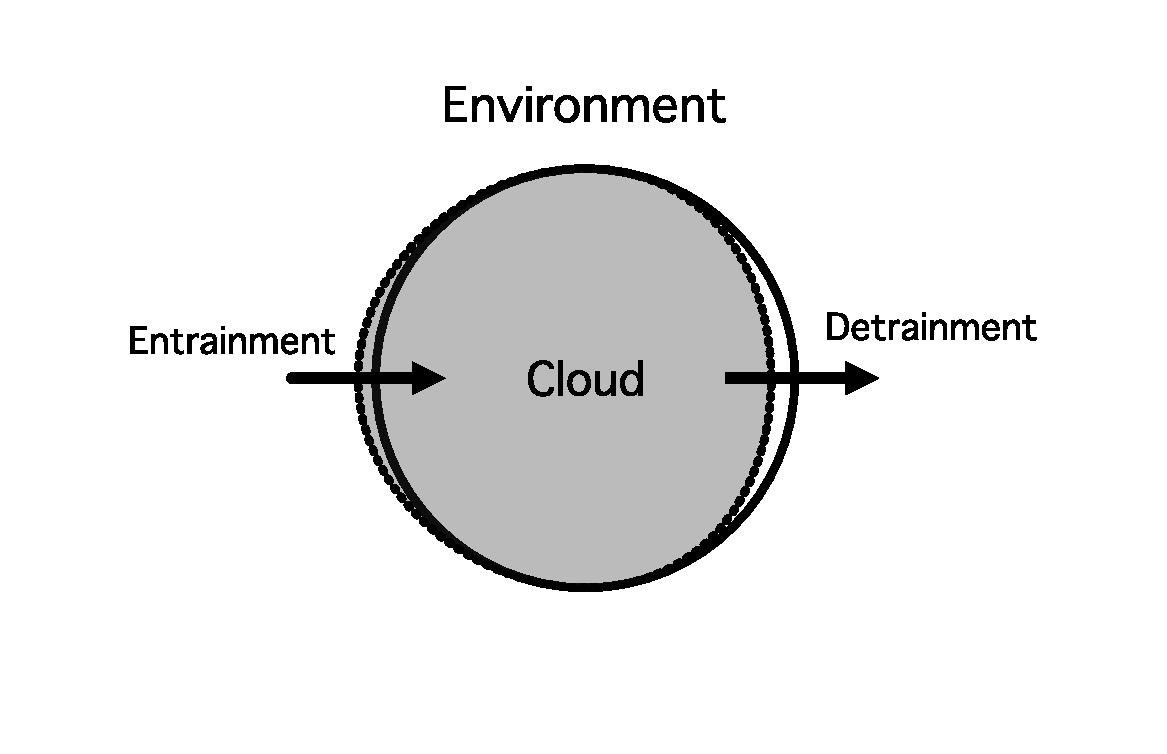
\includegraphics[width=0.7\textwidth]{img/ed.pdf}
        \caption{ An Overview of Entrainment and Detrainment Processes }
    \end{figure}
    Due to mixing between the cloud and the environment, the surrounding air is \emph{entrained} into the cloud and the cloudy air gets \emph{detrained} to the environment.
\end{frame}

\begin{frame}
    \frametitle{Mass Flux}
    Entrainment and detrainment rates, e and e, contribute to the changes in cloud mass flux $M_c = \rho w a$; that is,
    \begin{equation}
        \frac{\partial M_c}{\partial z} = e - d
    \end{equation}
    from which vertical distributions of cloud mass, heat, moisture and momentum can be obtained.
\end{frame}

\begin{frame}
    \frametitle{Representation of Clouds}
    In large-scale models, individual cloud effects cannot be resolved:
    \begin{figure}
        \centering
        \begin{minipage}{.5\textwidth}
            \centering
            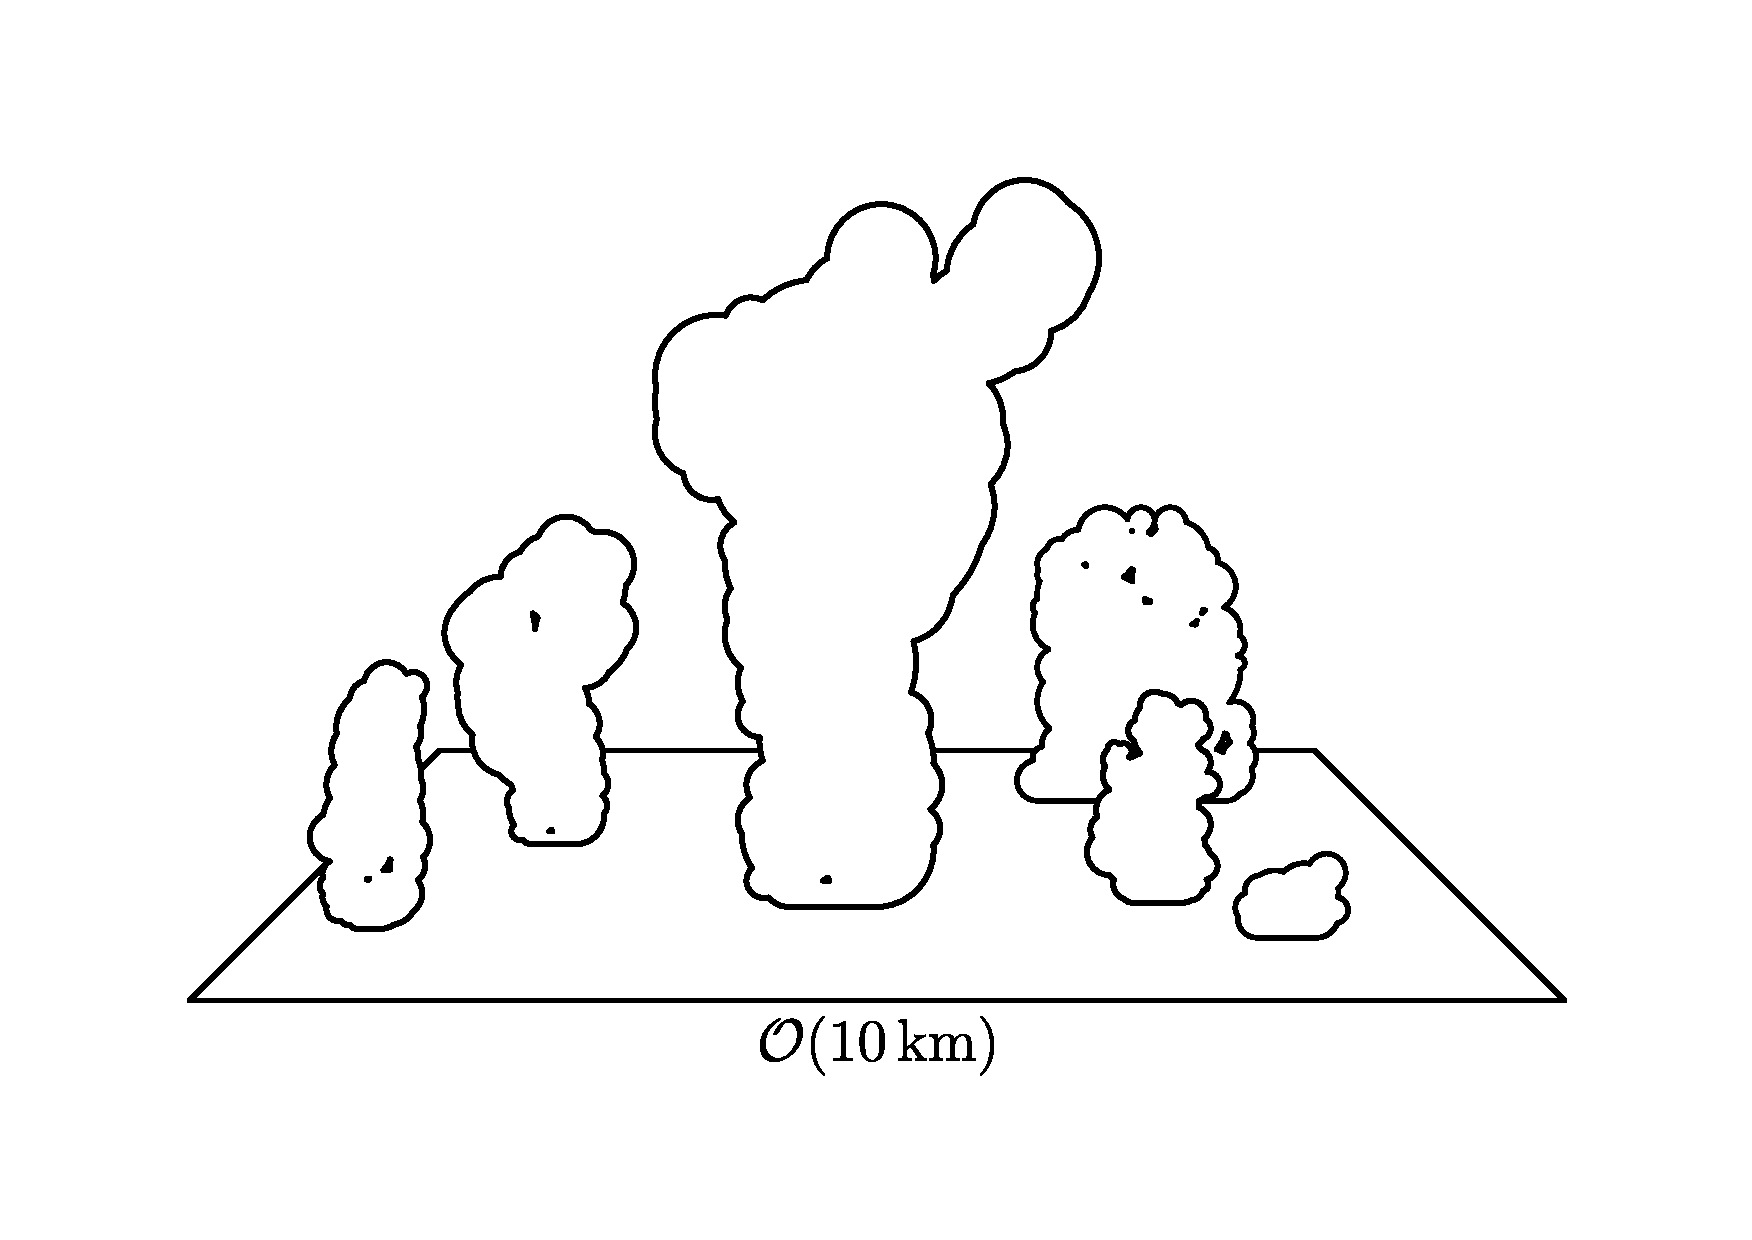
\includegraphics[width=\linewidth]{img/field.pdf}
            \caption{GCMs and NWPs}
        \end{minipage}%
        \begin{minipage}{.5\textwidth}
            \centering
            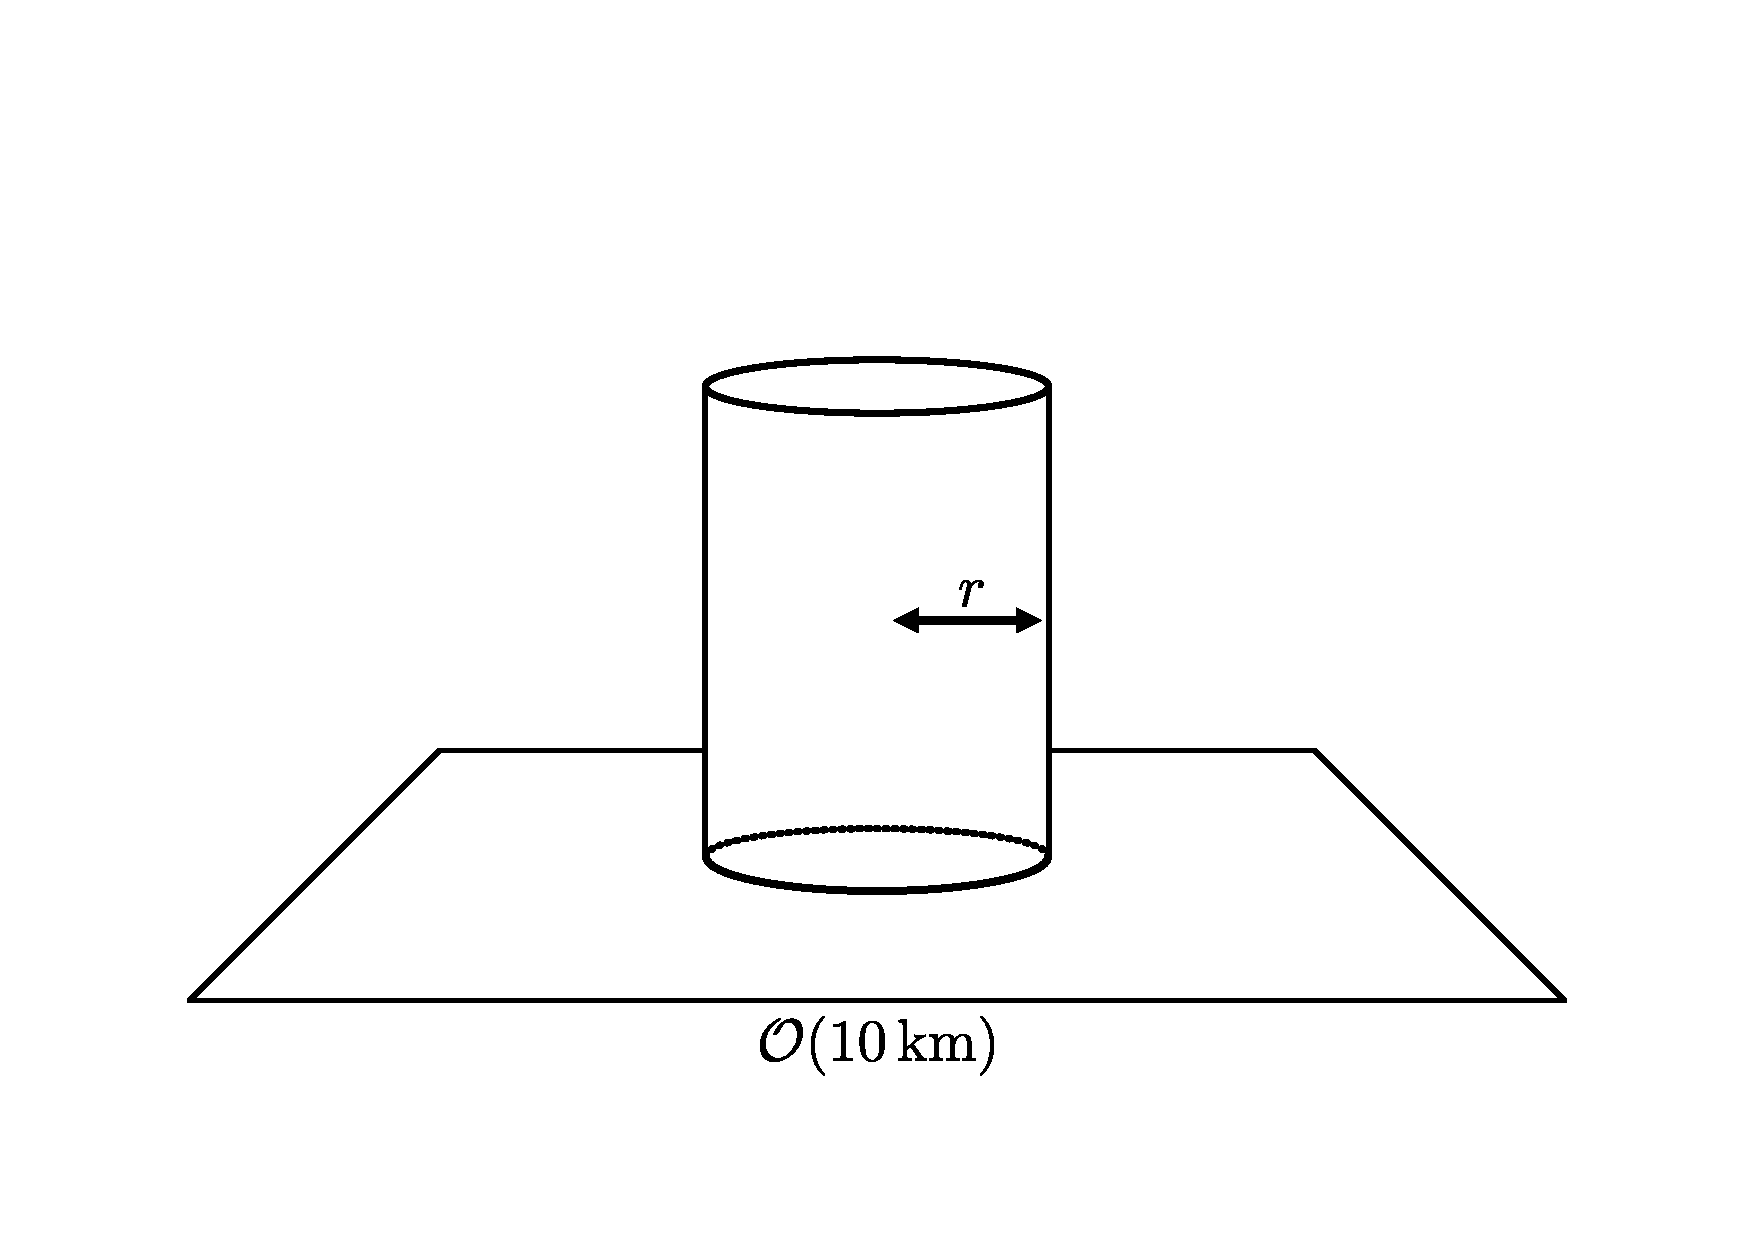
\includegraphics[width=\linewidth]{img/cyl.pdf}
            \caption{Bulk-plume Approximation}
        \end{minipage}
    \end{figure}
    The single \emph{bulk-plume} represents all clouds in the domain.
\end{frame}

\begin{frame}
    \frametitle{Bulk-plume Representation}
    For an arbitrary cloud tracer $\phi$,
    \begin{equation}
        e_b \overline{\phi} - d_b \phi_c =
            + \rho \frac{\partial \sigma \phi_c}{\partial t}
            + \frac{\partial M_c \phi_c}{\partial z}
            + (F_\mathrm{turb})_c
            - \rho \sigma F_c
    \end{equation}
    Bulk-plume estimates of entrainment and detrainment rates $e_b$ and $d_b$ are obtained as a residual of changes in cloud mass.
\end{frame}

\begin{frame}
    \frametitle{Direct Calculation of Entrainment and Detrainment Rates}
    \begin{figure}
        \centering
        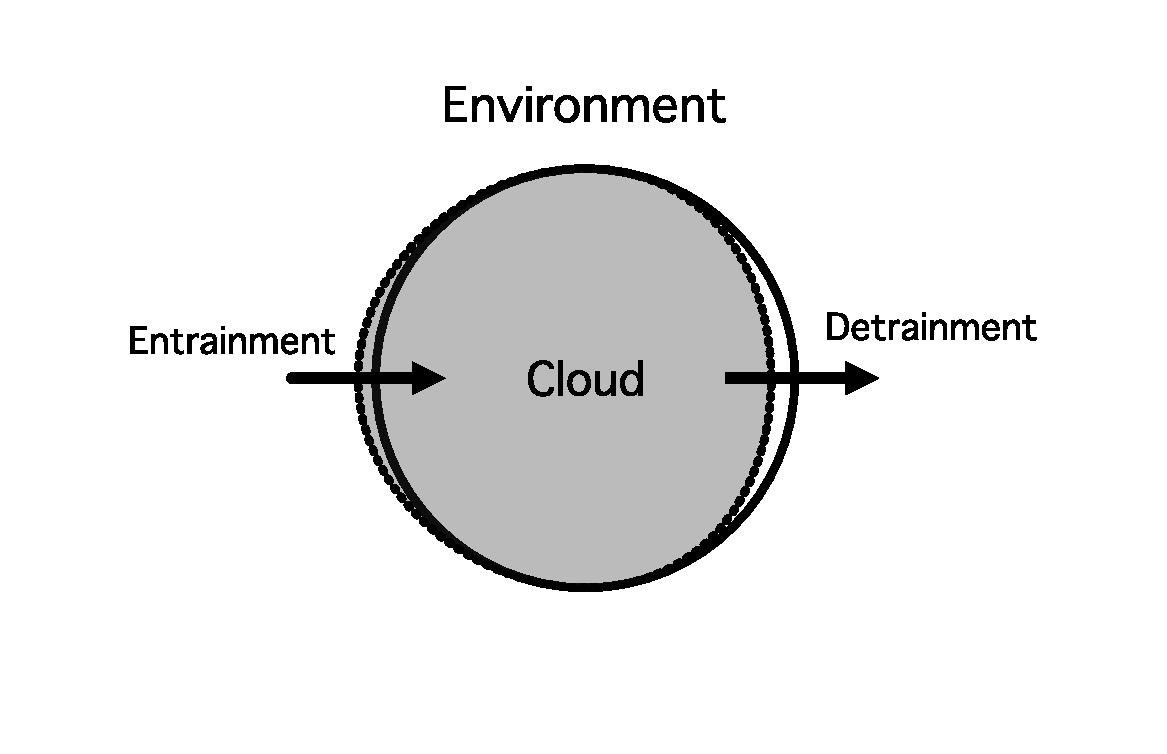
\includegraphics[width=0.7\textwidth]{img/ed.pdf}
        \caption{ An Overview of Entrainment and Detrainment Processes }
    \end{figure}
    Numerically, entrainment and detrainment events correspond to changes in cloud boundaries.
\end{frame}

\begin{frame}
    \frametitle{Direct Calculation of Entrainment and Detrainment Rates}
    \begin{figure}
        \centering
        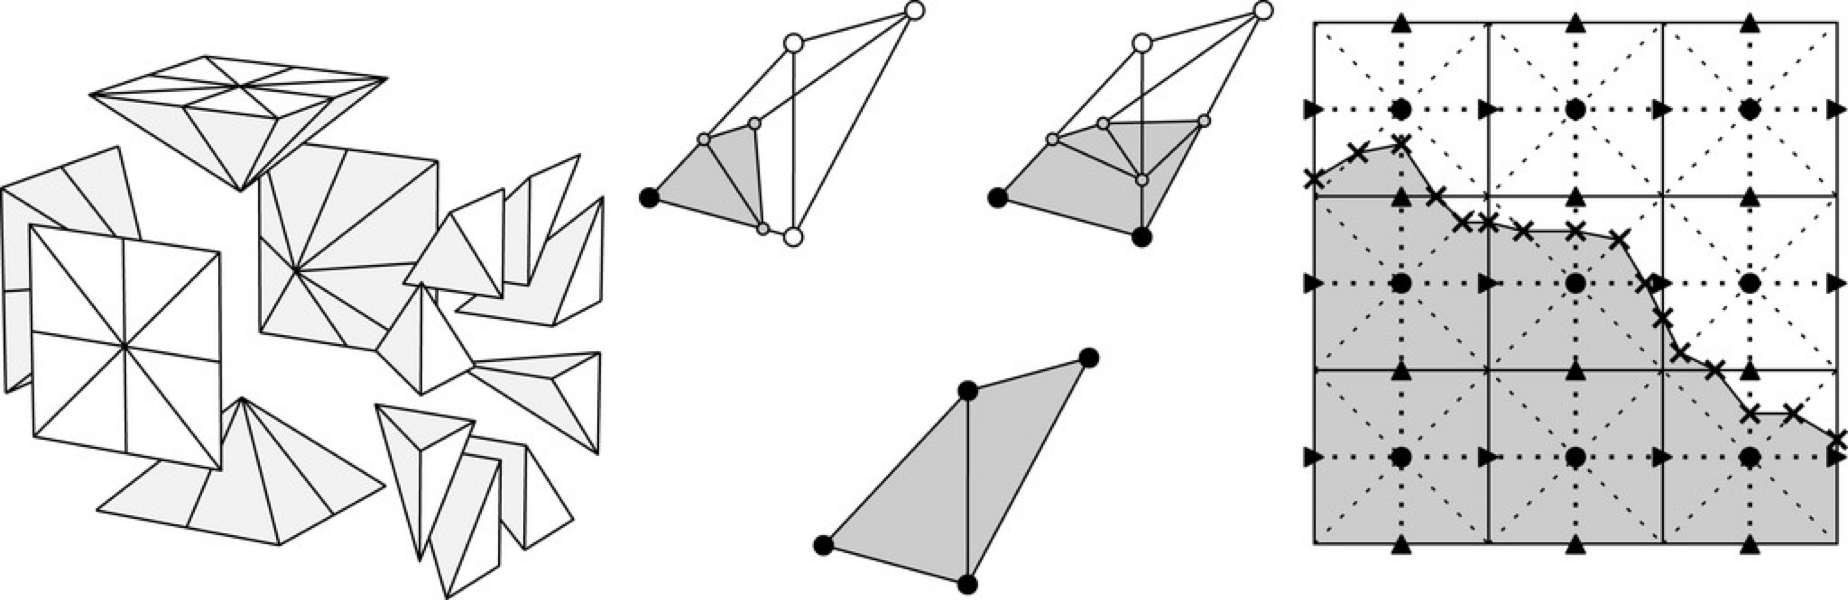
\includegraphics[width=0.95\textwidth]{img/tetra.png}
        \caption{ Tetrahedral Interpolation Scheme }
    \end{figure}
    Instead, entrainment and detrainment rates can be calculated directly by numerical techniques to track the changes in subgrid-scale changes in cloud volume (Dawe and Austin, 2011a).
\end{frame}

\begin{frame}
    \frametitle{Large-eddy Simulation}
    \begin{figure}
        \centering
        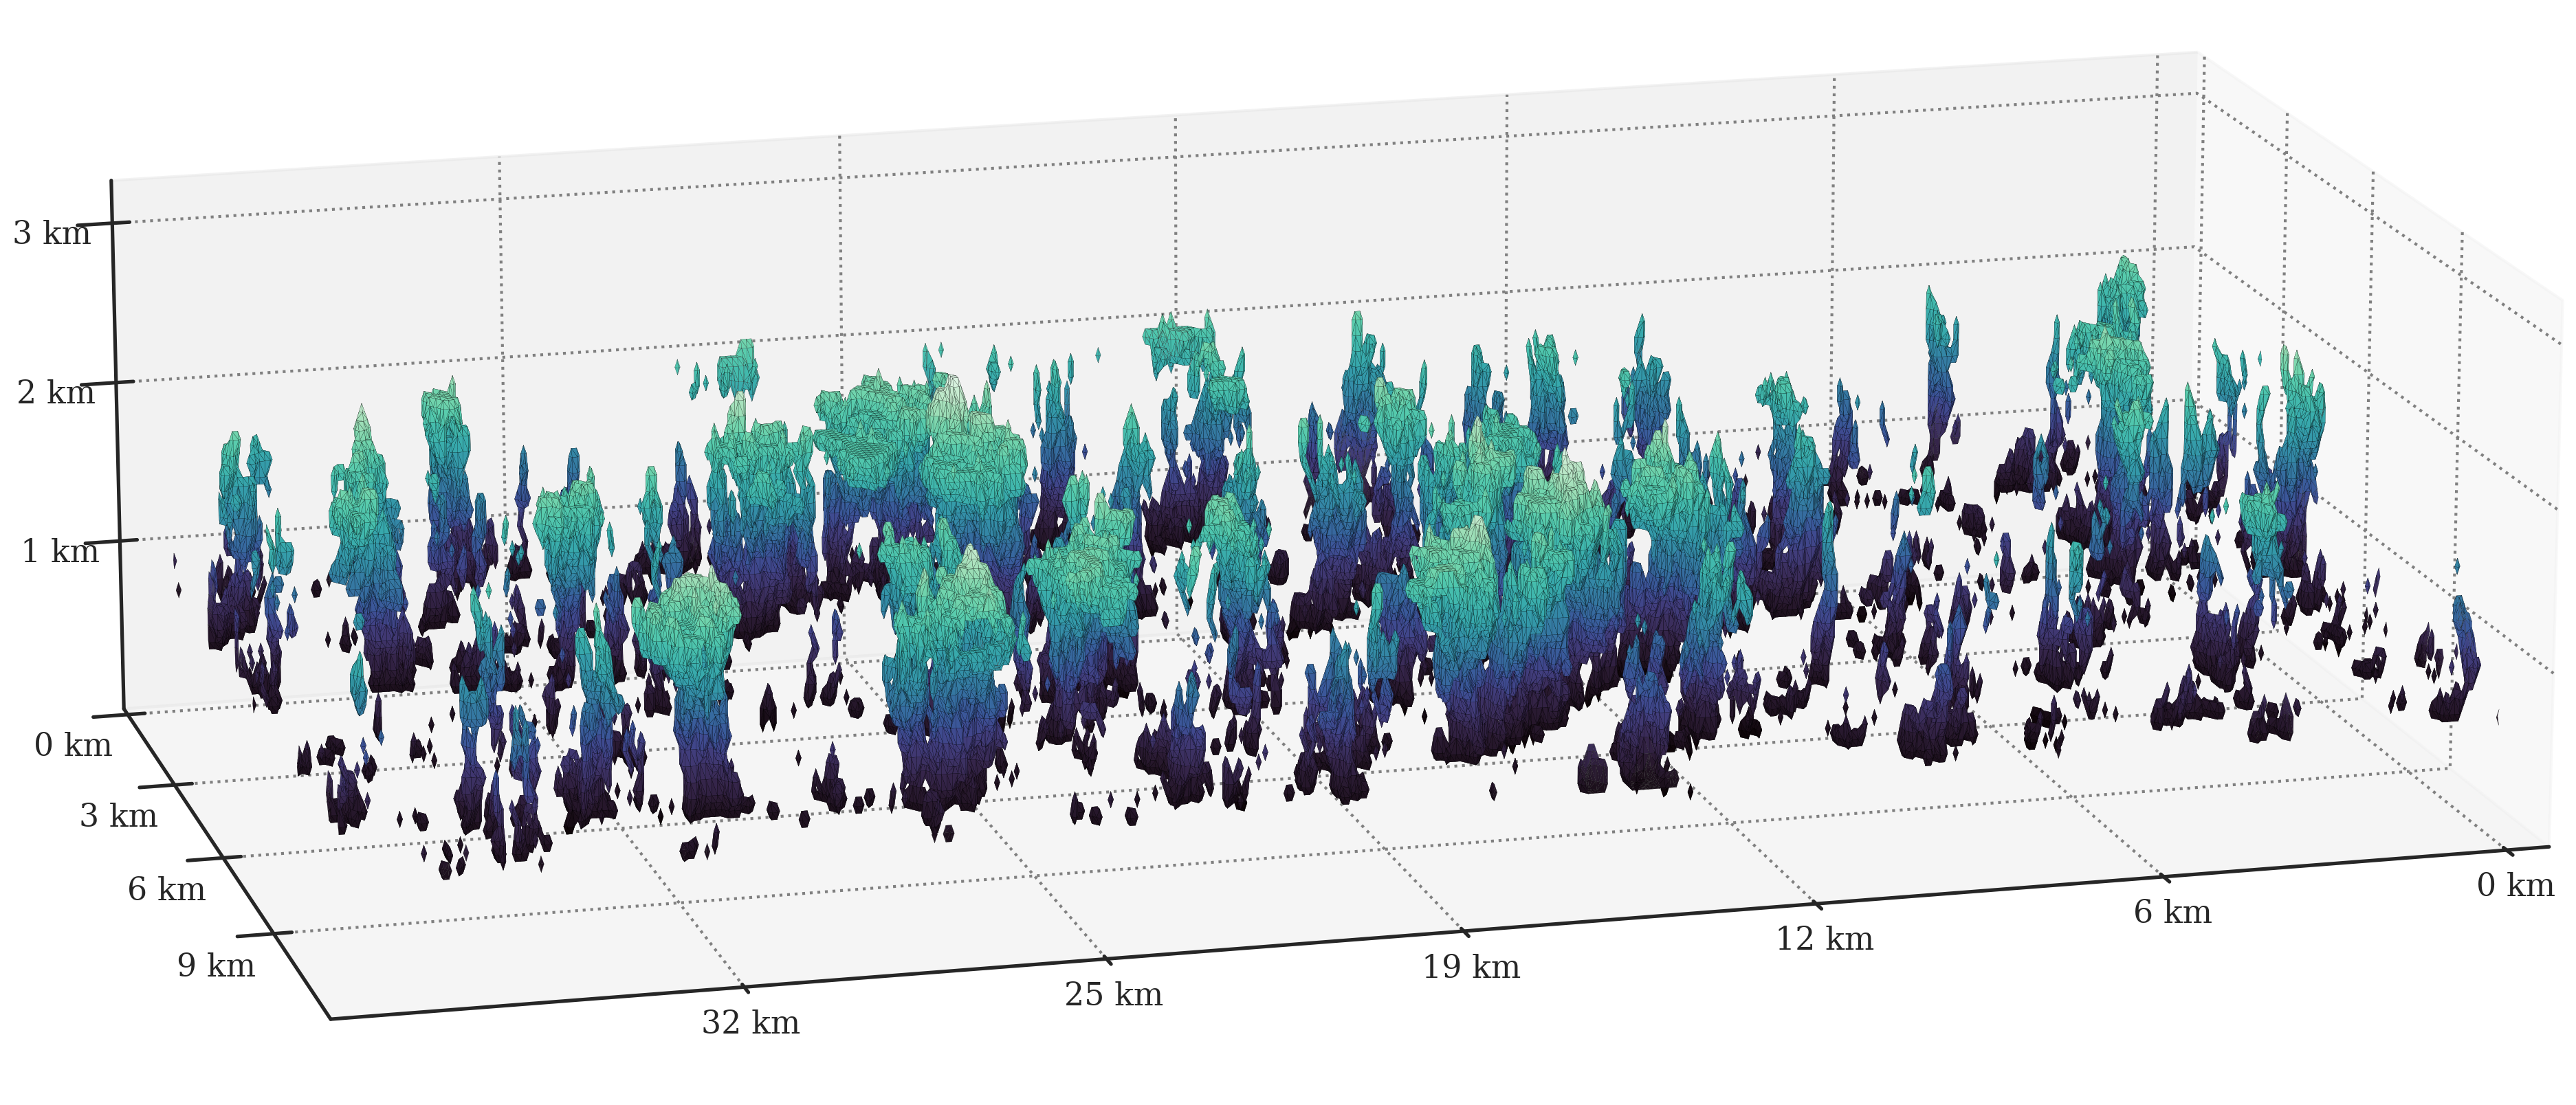
\includegraphics[width=\textwidth]{img/les.png}
        \caption{ A Snapshot from the LES Model Run }
    \end{figure}
    The System for Atmospheric Modelling (SAM)

    38.4 km $\times$ 12.8 km $\times$ 42 km domain with 25 m resolution
\end{frame}

\begin{frame}
    \frametitle{Cloud Mass Continuity Equations}
    We can write continuity equations for the cloud field as
    \begin{align}
        \label{eq:mam}
        \frac{D}{D t} \langle \rho \rangle &= \langle e \rangle - \langle d \rangle
        \\
        \label{eq:mpm}
        \frac{D}{D t} \langle \rho \phi \rangle &= \langle e \phi \rangle - \langle d \phi \rangle + \langle S_\phi \rangle
    \end{align}
    where $\langle \rangle$ denotes summation over the cloud field
\end{frame}

\begin{frame}
    \frametitle{Cloud Field Net Entrainment}
    \begin{figure}
        \centering
        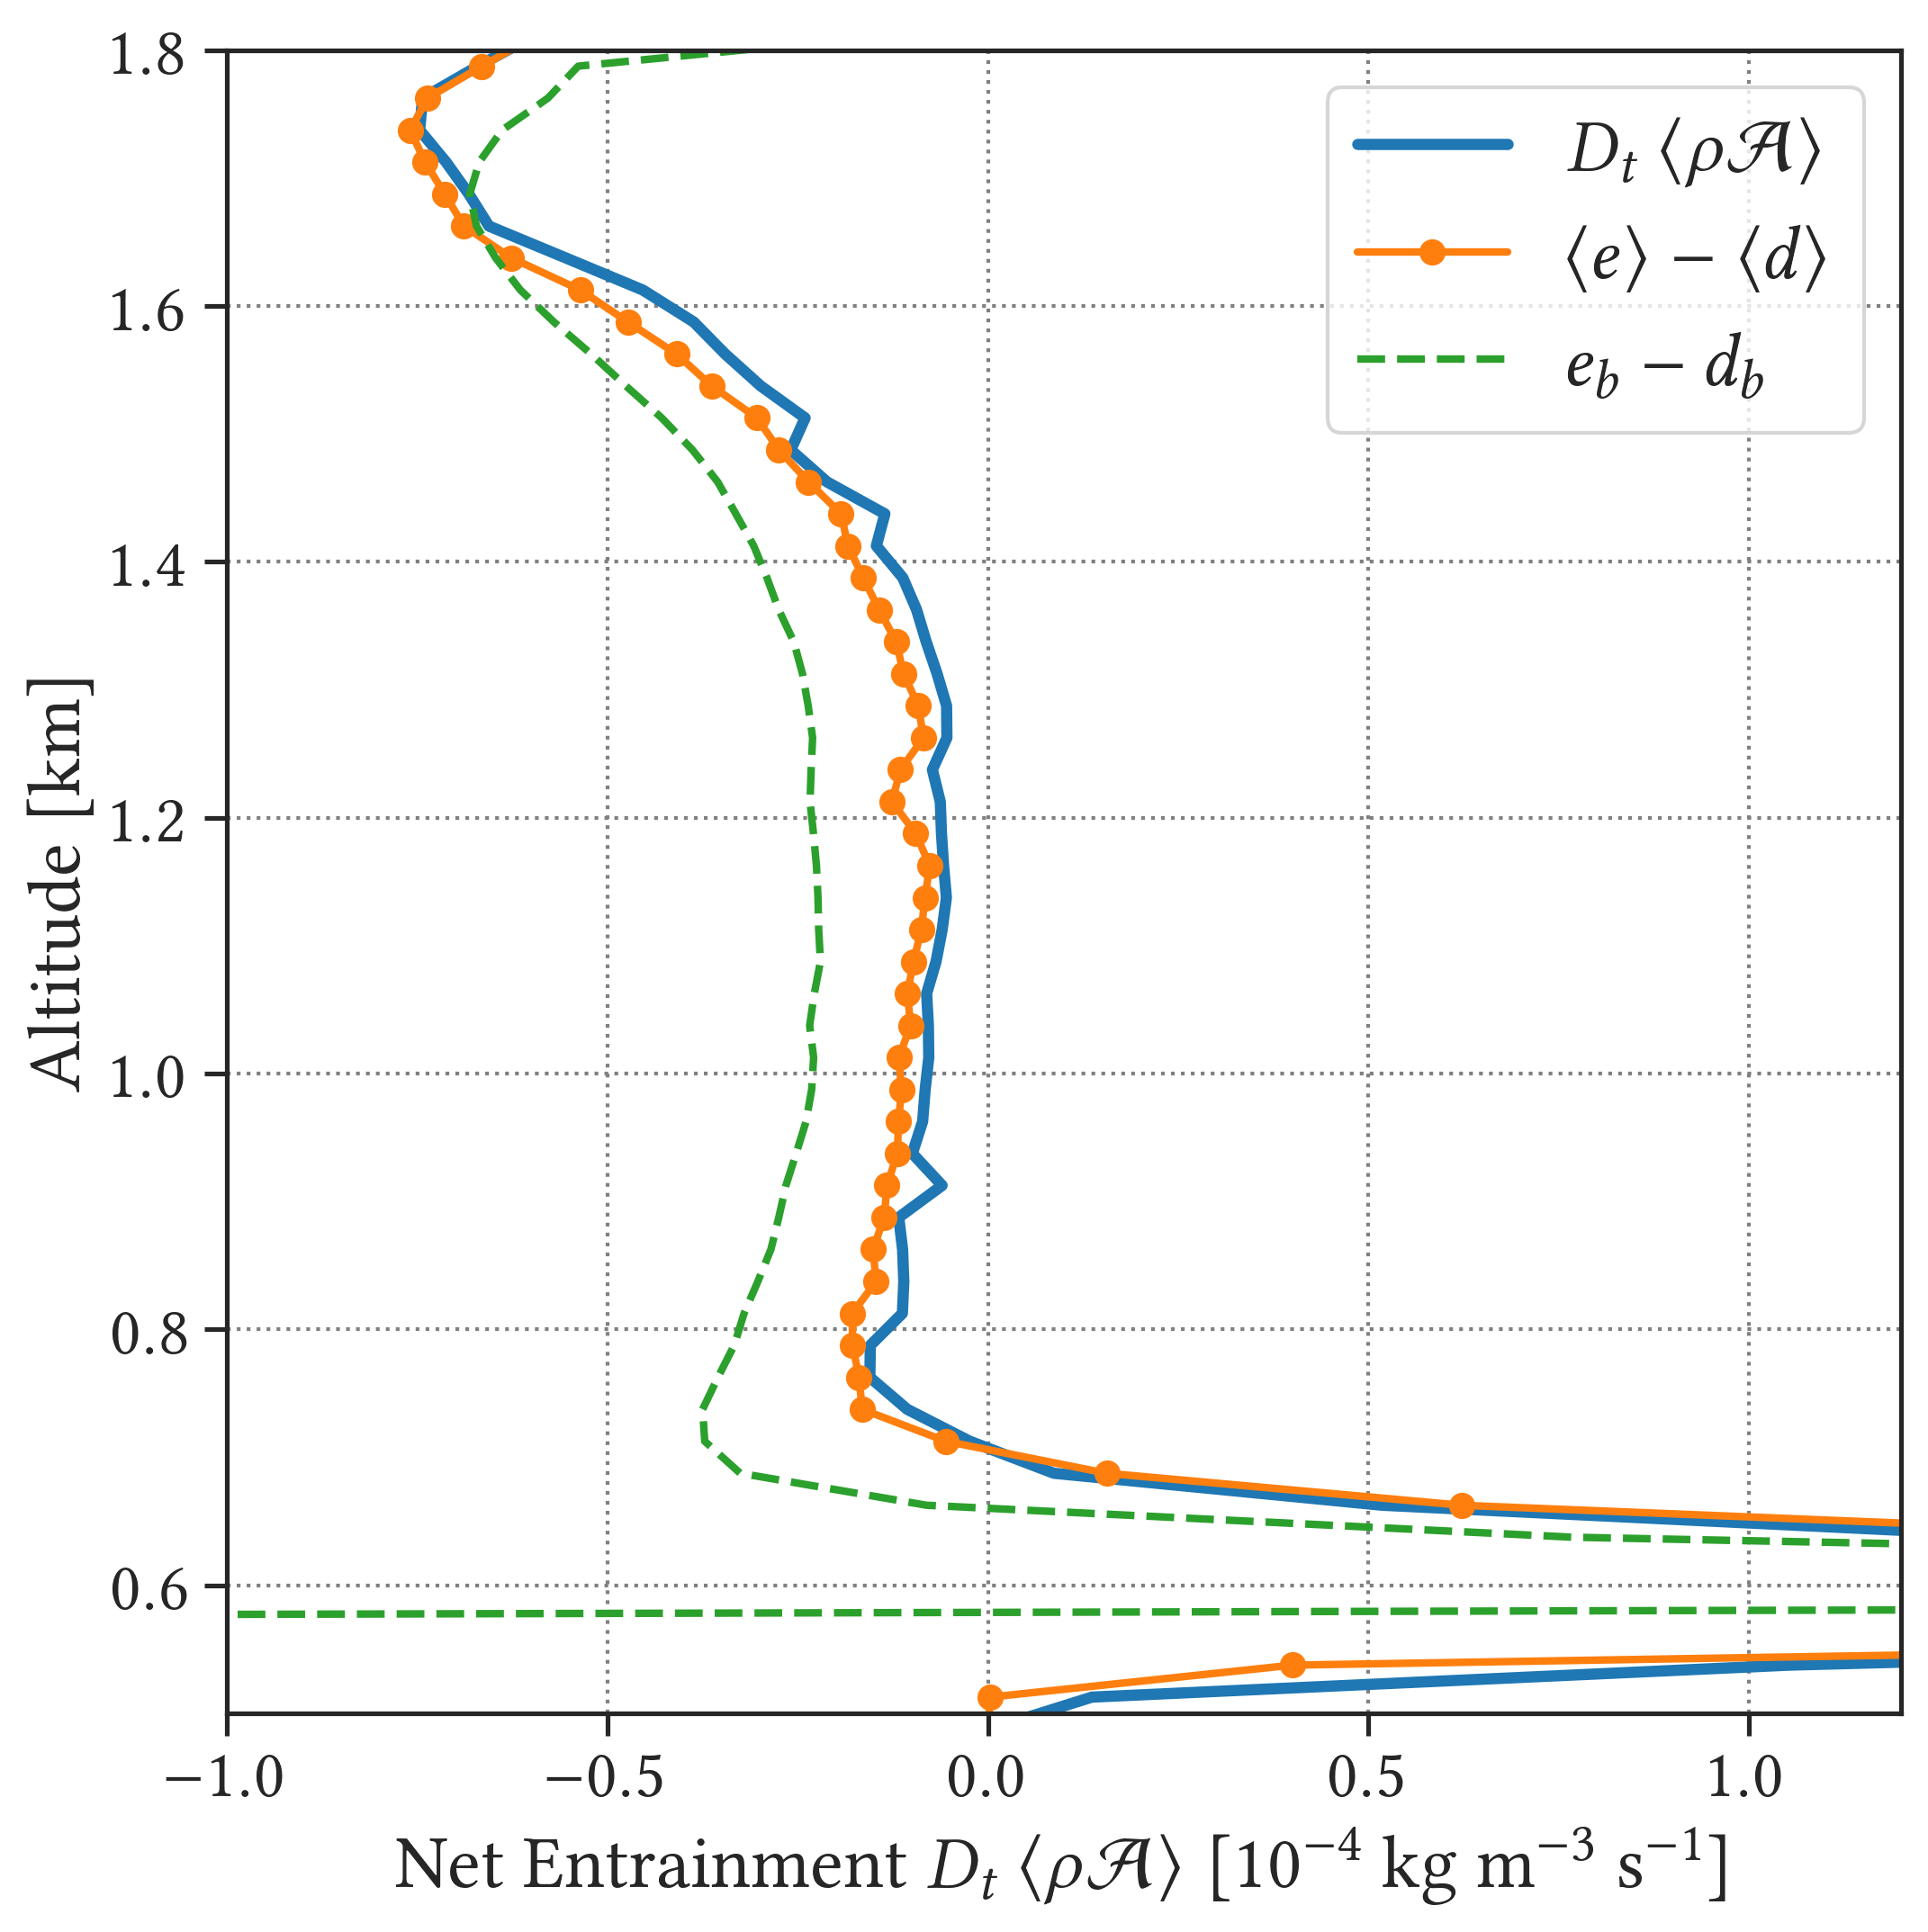
\includegraphics[width=0.6\textwidth]{img/nent.png}
        \caption{ Net Entrainment Rate for the LES-modelled Cloud Field }
    \end{figure}
\end{frame}

\begin{frame}
    \frametitle{Cloud Sampling}
    \begin{figure}
        \centering
        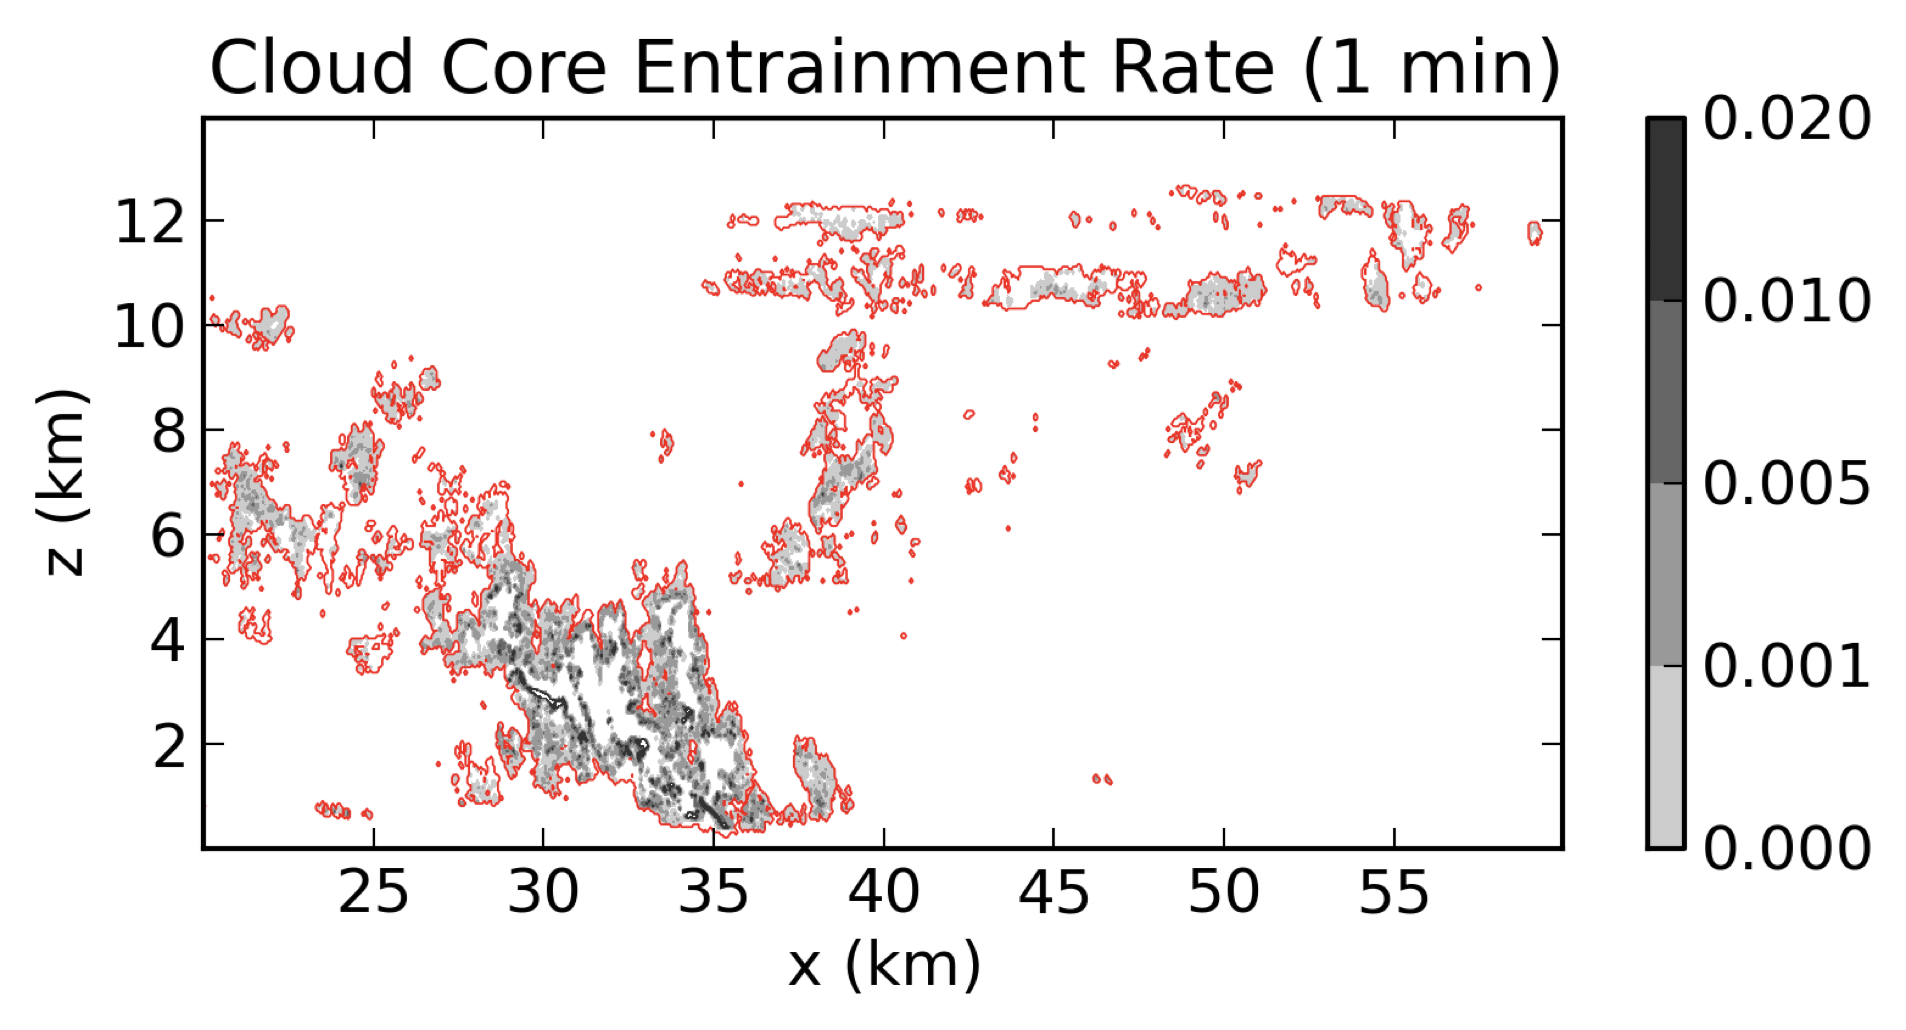
\includegraphics[width=0.9\textwidth]{img/core.png}
        \caption{ A Snapshot from the LES Model Run }
    \end{figure}
    Identify cloud region containing condensed liquid water
\end{frame}

\begin{frame}
    \frametitle{Cloud Sampling}
    \begin{figure}
        \centering
        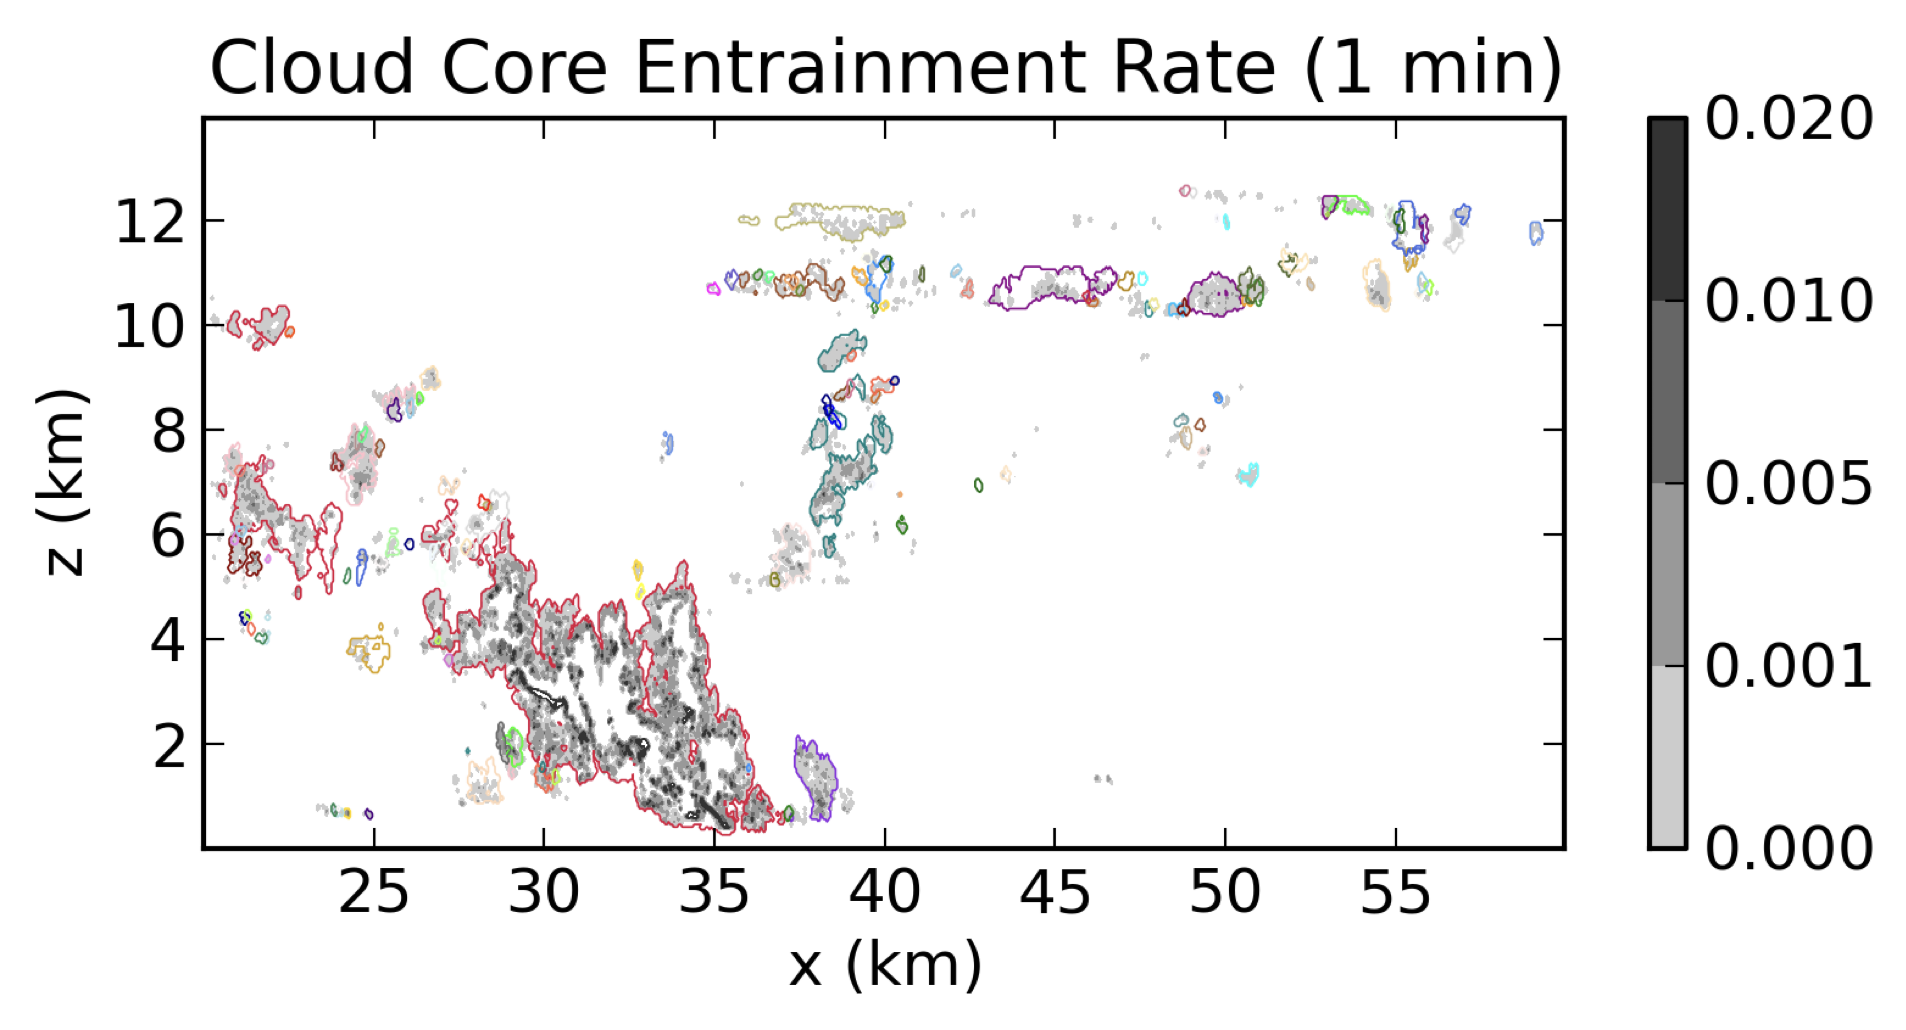
\includegraphics[width=0.9\textwidth]{img/cores.png}
        \caption{ A Snapshot from the LES Model Run }
    \end{figure}
    Individual cloud properties show large variability.
\end{frame}

\begin{frame}
    \frametitle{Individual Cloud Properties}
    \begin{figure}
        \centering
        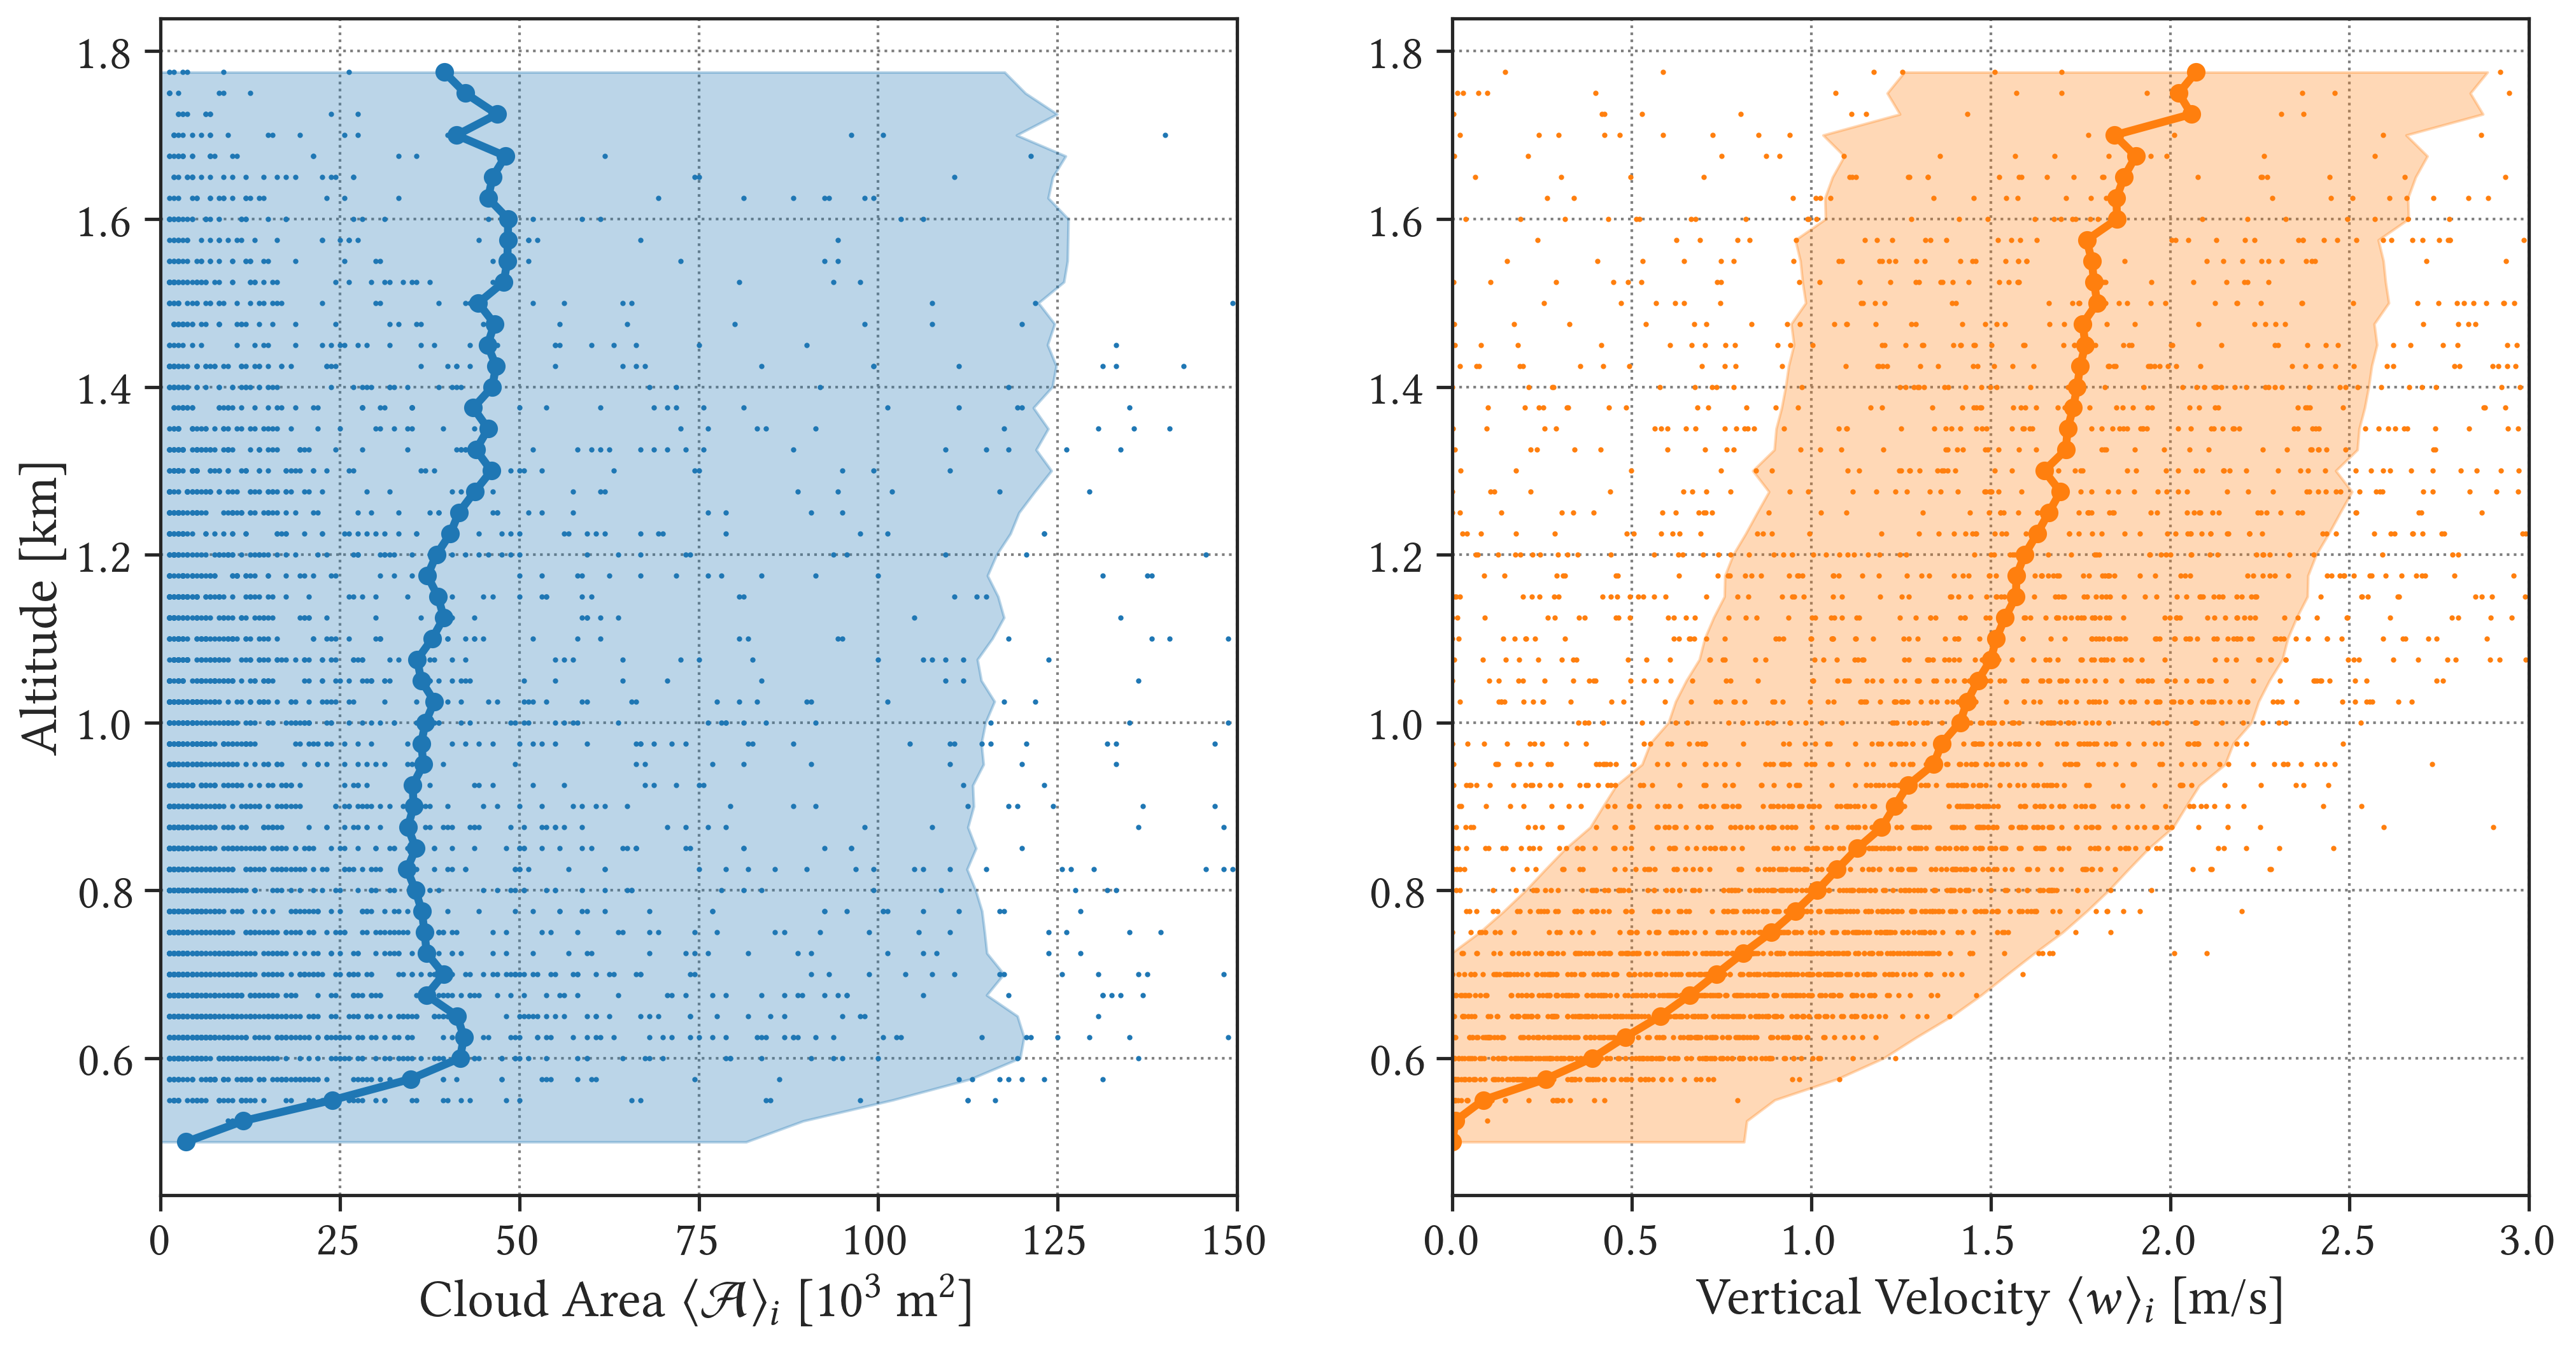
\includegraphics[width=0.8\textwidth]{img/aw.png}
        \caption{ Individual Cloud Area (left) and Vertical Velocity (right) }
    \end{figure}
    Sample individual clouds as contiguous regions
\end{frame}

\begin{frame}
    \frametitle{Proportional Dilution Rate}
    Proportional changes in tracer tracer $\phi$ can be fully quantified by continuity equations:
    \begin{align}
        \frac{\langle \rho \rangle _i}{\langle \rho \phi' \rangle _i} \frac{D}{D t} \phi_c
        &= \frac{1}{\langle \rho \phi' \rangle _i} \left\{ \left( \frac{D}{D t} \langle \rho \phi \rangle _i \right) - \phi_c \left( \frac{D}{D t} \langle \rho \rangle _i \right) \right\}
        \\
        &= \frac{1}{\langle \rho \phi' \rangle _i} \left\{ - \langle e \rangle _i (\phi_c - \phi_e) + \langle d \rangle _i (\phi_c - \phi_d) + \langle \rho S_\phi \rangle _i \right\}
    \end{align}
    where $\langle \rangle _i$ denotes summation individual clouds
\end{frame}

\begin{frame}
    \frametitle{Proportional Dilution Rate}
    \begin{figure}
        \centering
        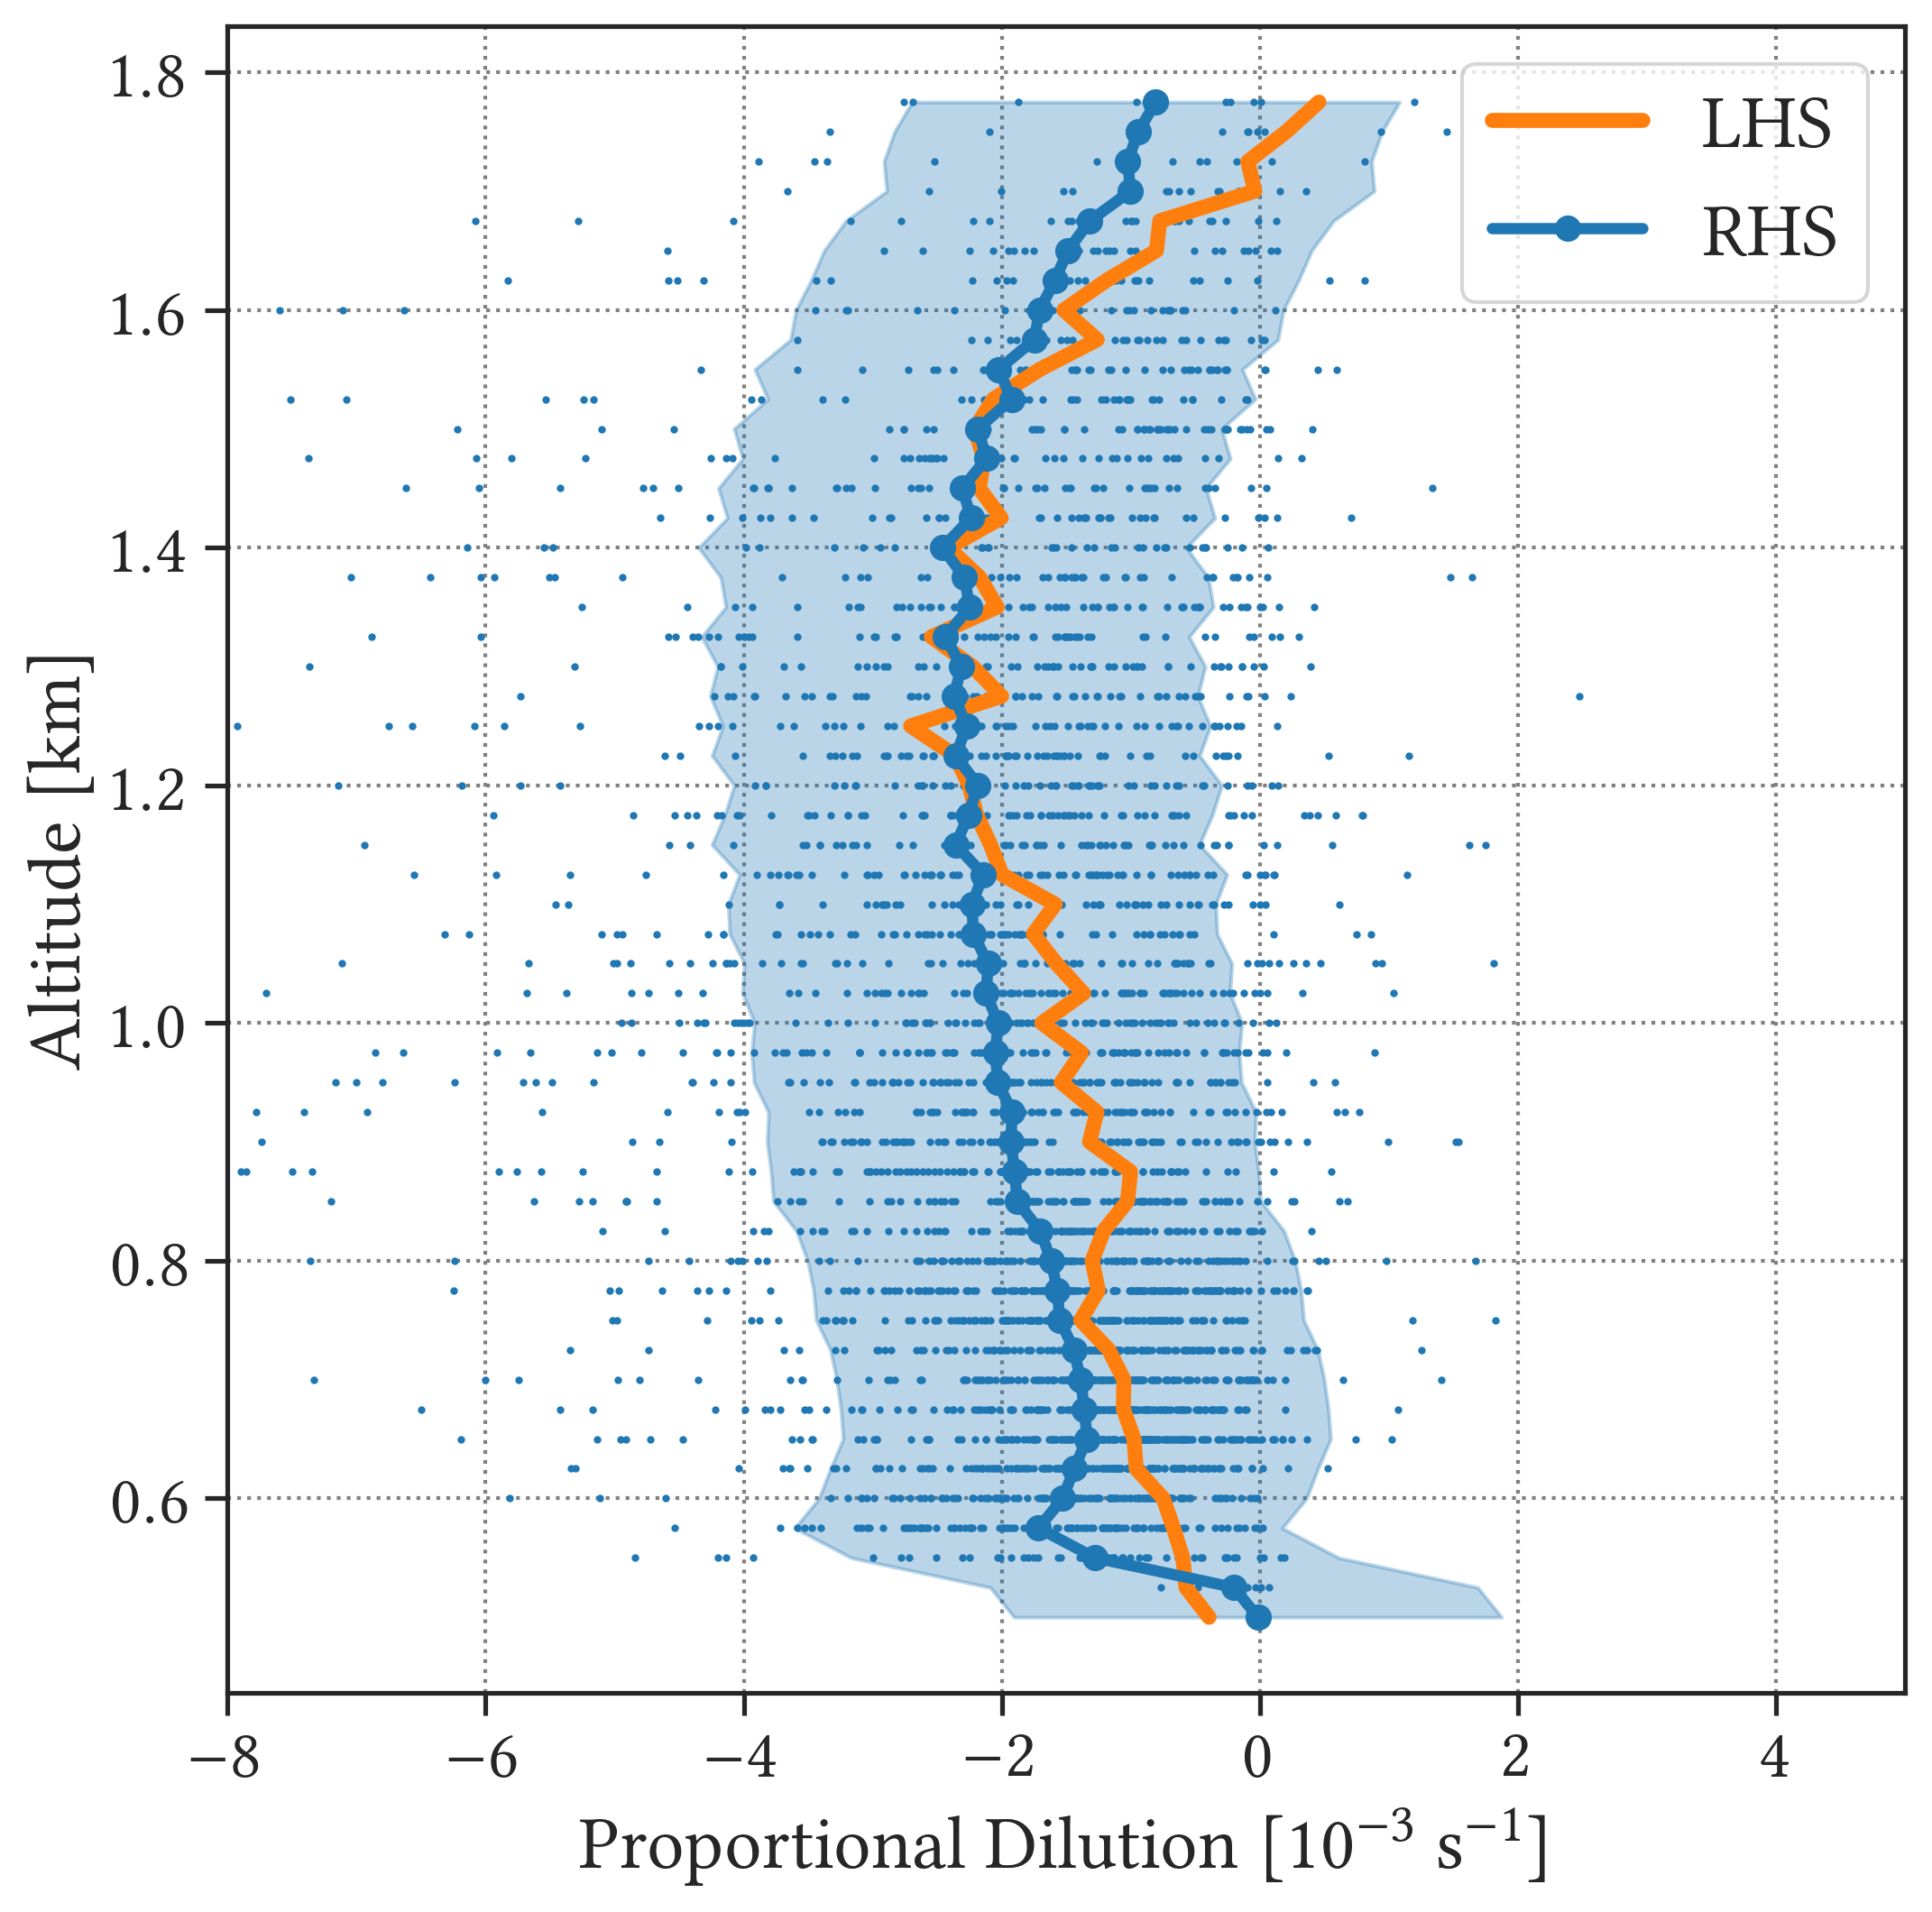
\includegraphics[width=0.6\textwidth]{img/ndil.png}
        \caption{ The Rate of Proportional Dilution for Individual CLouds }
    \end{figure}
\end{frame}

\begin{frame}
    \frametitle{Direct Calculation of Entrainment and Detrainment Rates}
    \begin{figure}
        \centering
        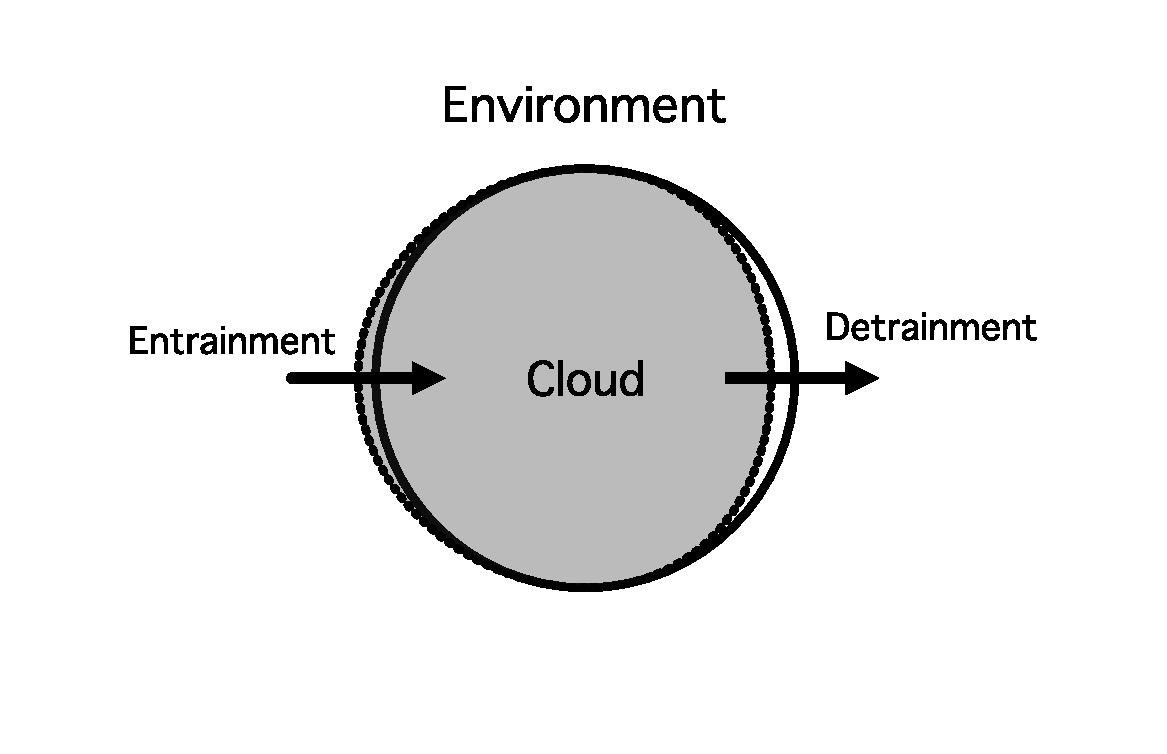
\includegraphics[width=0.7\textwidth]{img/ed.pdf}
        \caption{ An Overview of Entrainment and Detrainment Processes }
    \end{figure}
    The bulk-plume approximation makes an assumption that the cloud field as a whole mixes directly with the dry environment.
\end{frame}

\begin{frame}
    \frametitle{Moist Shell}
    \begin{figure}
        \centering
        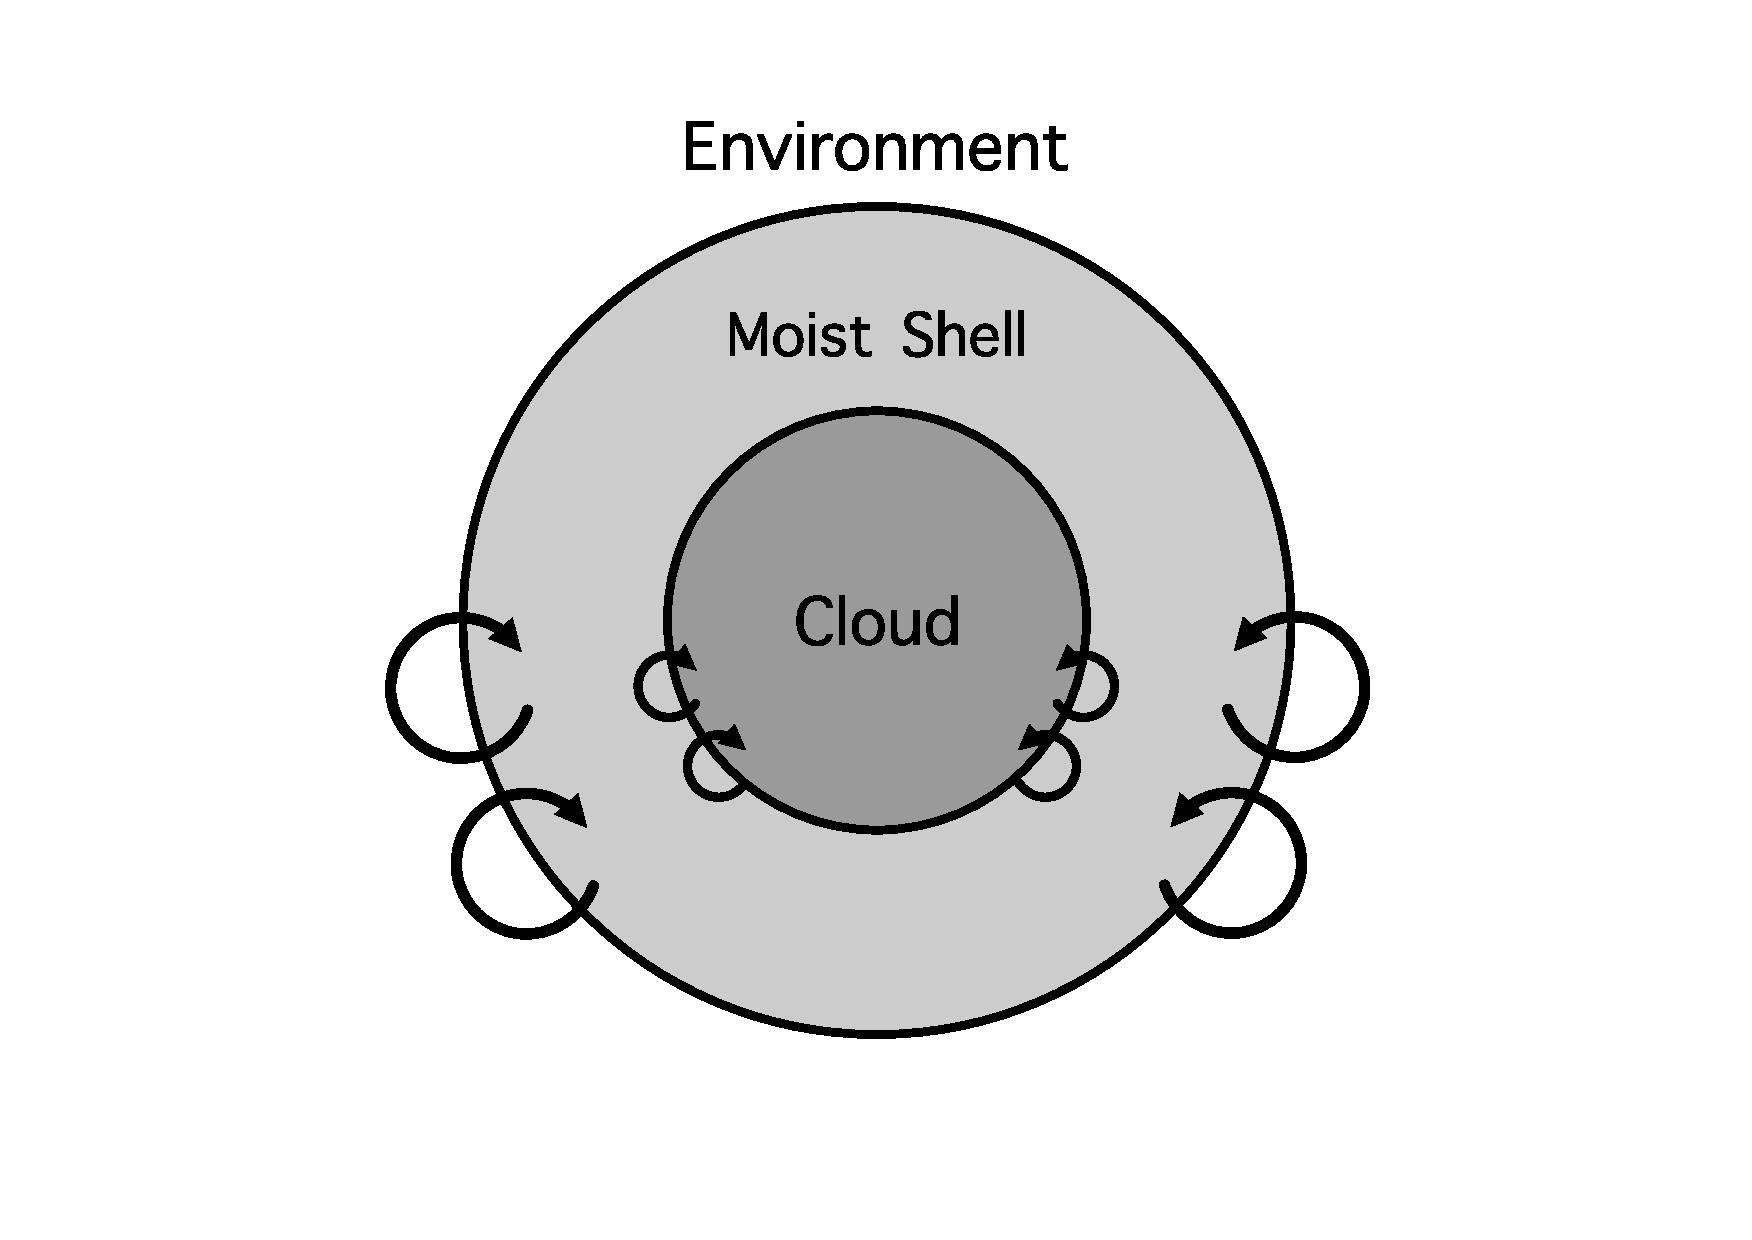
\includegraphics[width=0.6\textwidth]{img/shell.pdf}
        \caption{ A Diagram for the Moist Shell }
    \end{figure}
    Individual cloud regions are surrounded by a shell of moist air modulating the turbulent mixing between the clouds and their surroundings.
\end{frame}

\begin{frame}
    \frametitle{Remarks}
    \begin{align*}
        \frac{\langle \rho \rangle _i}{\langle \rho \phi' \rangle _i} \frac{D}{D t} \phi_c
        &= \frac{1}{\langle \rho \phi' \rangle _i} \left\{ \left( \frac{D}{D t} \langle \rho \phi \rangle _i \right) - \phi_c \left( \frac{D}{D t} \langle \rho \rangle _i \right) \right\}
        \\
        &= \frac{1}{\langle \rho \phi' \rangle _i} \left\{ - \langle e \rangle _i (\phi_c - \phi_e) + \langle d \rangle _i (\phi_c - \phi_d) + \langle \rho S_\phi \rangle _i \right\}
    \end{align*}
    We introduce a principled approach to fully quantify the tendencies of cloud mass and tracer concentration $\phi$.

    Numerical methods are shown to be able to precisely reproduce these tendencies at the LES scale.
\end{frame}

\end{document}